\chapter{\diva general theory\label{chaptheory}}
%TEST

This chapter describes the theory behind the \diva interpolation method and compares it with the Optimal Interpolation. 

\minitoc


\section{The gridding problem\label{gridding}}
%----------------------------------------------

The generation of gridded fields from non-uniformly distributed observations (both in space and time) is a frequent concern in geosciences. Similarly to \citet{OOYAMA87}, we will refer to an \textit{analysis} or \textit{analysed field} as "the estimation of a continuous spatial field of a given variable from a set of discrete measurements". The range of applications is wide, going from model initializations to validation exercises  or simple plotting purposes. 

Mathematically, gridding consists in determining a field $\varphi(\mathbf{r})$ on a regular grid at positions $\mathbf{r}$, using $N_{d}$ measurements located in $\mathbf{r_{j}}, j=1,\ldots, N_{d}$ (Fig.~\ref{gridproblem}).  

In this chapter we consider only two-dimensional cases, but generalization can be done to $3$D and even $4$D (using "distance" in time, but being aware of autocorrelations as in seasonal signals).

\begin{figure}[htpb]
	\centering
	\parbox{.5\textwidth}{
		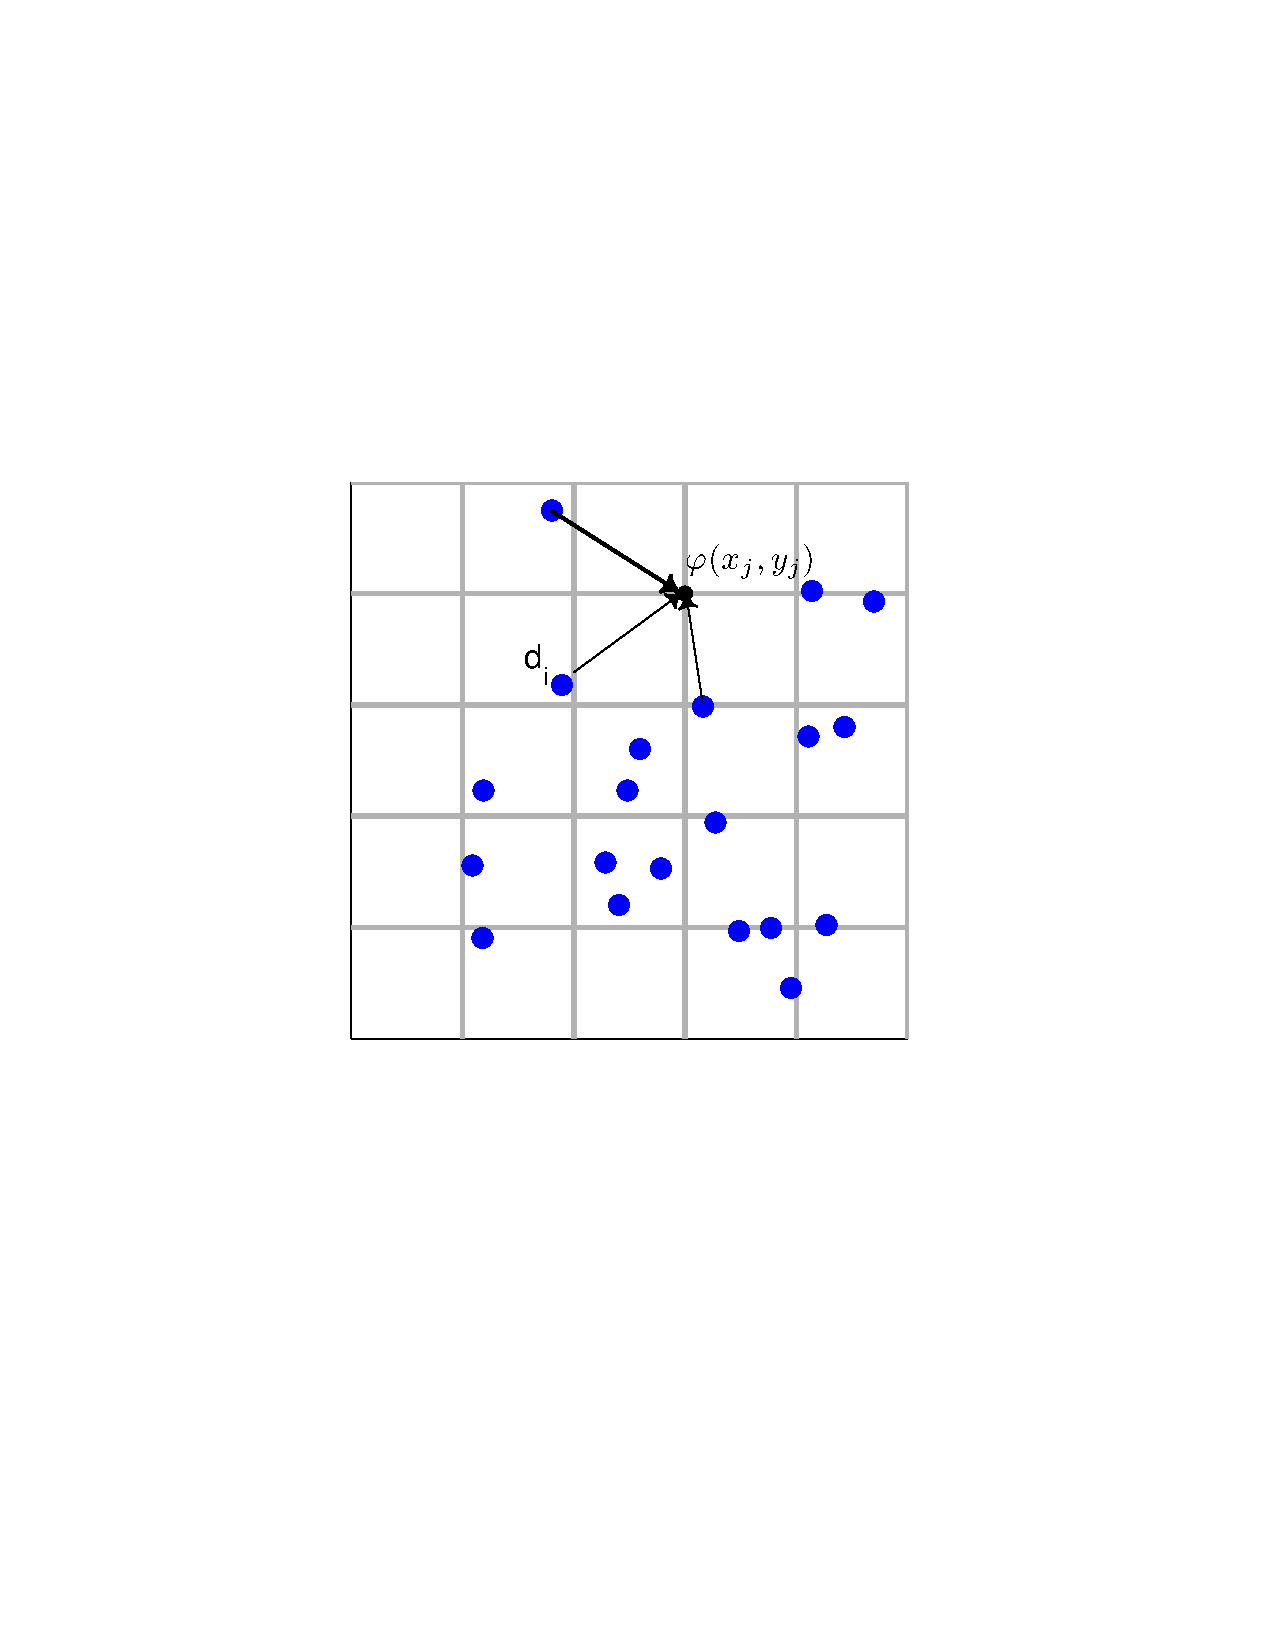
\includegraphics[width=.45\textwidth,bb=166  289 440 564]{gridding}
		}\parbox{.5\textwidth}{
		\caption{Gridding problem: the blue dots indicate data positions, while the nodes of the grid  are the points where the field has to be determined.\label{gridproblem}}
		}
\end{figure}

%----------------------------------------------
\subsection{Interpolation versus approximation}
%----------------------------------------------

For solving the gridding problem, two main techniques have to be distinguished:

\begin{enumerate}

\item The \textit{interpolation}, which implies a strict passage of the solution through the points of data. Physically, this means that one assumes that there is no error on the data. 

% Among the methods of interpolation, let us mention: the linear, cubic, inverse distance, optimal interpolations, the \textit{kriging}, \ldots

\item The \textit{approximation} (or \textit{analysis}) provides a solution smoother than the one given by interpolation: in this case, the solution does not necessarily have to contain all the data points. The solution is close to the data points, so its shape is still influenced by the data. This technique allows taking into account errors on data, as well as to treat multiple data with different values at the same location. 
\end{enumerate}

\begin{figure}[htpb]
	\centering
	\parbox{.5\textwidth}{
		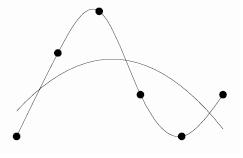
\includegraphics[width=.35\textwidth]{approx}
		}\parbox{.5\textwidth}{
		\caption{Interpolation provides a solution that goes across all the data points, while the approximation has only to be "close" to the measurements, but with a relative "smoothness".}
		}
\end{figure}


\subsection{Objective versus subjective data analysis methods\label{sec:gridding}}
% --------------------------------------------------------------------------------

In geosciences and in particular in oceanography, it is frequent to have error on the measurements and close data points. Hence the approximation methods are preferred to strict interpolation techniques.

We have to differentiate \textit{subjective} analysis, for which the way the approximation is performed is decided by hand, and \textit{objective} analysis, which is based on predefined mathematical operations. Note that beyond these two kinds of analysis, \textit{data assimilation} uses in addition physical/biochemical dynamic governing equations. 

Since data assimilation depends on the region and the model and the subjective analysis is not sufficiently objective, the objective analysis is chosen here. 

%------------------------------------------
\subsection{Background field and anomalies}
%------------------------------------------

\index{Background field}
The field $\varphi(\mathbf{r})$ can be decomposed as the sum of a \textit{background field} \index{Background field} $\varphi_b$ and an anomaly $\varphi'$: 
\begin{equation}
 \varphi(\mathbf{r}) = \varphi_b(\mathbf{r}) + \varphi'(\mathbf{r}).
 \label{background}
\end{equation}
Instead of working with the data themselves, we will work with the anomalies of these data with respect to the background field. The background field is defined a priori and the anomalies are calculated with respect to this reference field (e.g., climatological average, linear regression, theoretical solution). 

The anomalies are assumed to be computed as a linear combination of the data, i.e., 
\begin{equation}
\varphi(\mathbf{r}) = \varphi_b(\mathbf{r}) + \sum_{j=1}^{N_d} w_j\, d_j,
\label{objectiveanal}
\end{equation}
where $d_{j}$ is the data anomaly at $\mathbf{r}= \mathbf{r_{j}}$ and $w_j$ is the relative weight of the data $j$. The weighting functions are the new unknowns to determine: once the background field and the weighting functions are known, the field $\varphi$ can be computed at any position $\mathbf{r}$, hence gridding is possible.

From here on, we will work with anomaly only and therefore formally use $\varphi_{b}=0$.

% ------------------------
\subsection{Noise on data}
% ------------------------

\index{Noise}
When measuring a field, there is always an uncertainty on the value obtained (whatever the instrument and the field). \textit{Noise} \index{Noise} does not only take into account \textit{instrumental} error (which is generally low), but also:
\begin{itemize}
\item the \textit{representativeness} errors, meaning that what one measures is not always what ones intends to analyse):\\
e.g., skin temperature, inadequate scales, \ldots
\item the \textit{synopticity} errors, occuring when the measurements are assumed to be taken at the same time):\\
e.g., data from a cruise \citep{RIXEN01}.
\end{itemize}

Because of the multiple sources of error, a perfect fit to data is not advised, and the noise on the measurements has to be considered during the analysis.

%-------------------------------------------------------------
\section{The Optimal Interpolation method\label{sec:OImethod}}
%-------------------------------------------------------------
 
Before explaining the core of \diva technique, the main principles of \textit{Optimal interpolation} \citep[OI,][]{STOR99,CHILES99} are explained\index{OI}. OI is a popular analysis tool, owing to its ease of use and the error field associated to the analysis \citep[e.g.,][]{SHEN98b,KAPLAN00}. The first references of the method are \citet{GANDIN65} and \citet{BRETHERTON76}.

The idea is to minimise the expected error variance of the analysis. This conditions lead to the determination of the weights $w_j$ \eqref{objectiveanal}, with the assumption that the true anomaly field $\varphi_t$ is one realization out of a zero mean ensemble. 

Note that \textit{Kriging}\index{Kriging} \citep{KRIGE51,MATHERON63} is an equivalent technique: it uses the same criterion as OI, but with a different mathematical formulation: the weights $w_{j}$ are chosen from the study of the covariance between the values as a function of the distance between them.

%-------------------------------------
\subsection{Mathematical formulation}
%-------------------------------------

Let us recall previous notations from section \ref{gridding} and introduce some new ones:

$\varphi$, the interpolated (or reconstructed) field,\\
$\varphi_{t}$, the true (unknown) field,\\
$\mathbf{d}$, the vector containing the $N_{d}$ data,\\
$\mathbf{r}$, the vector position.

The principle of OI is to minimize the expected error:
\begin{equation}
e^{2}(\mathbf{r}) = \overline{[\varphi(\mathbf{r})-\varphi_{t}(\mathbf{r})]^{2}}
\end{equation}
where $\bar{\quad}$ stands for the statistical average.

Replacing the interpolated anomaly field by a linear combination of the data, we have 

\begin{equation}
e^{2}(\mathbf{r}) = \overline{\left[\sum_{i=1}^{N_{d}}w_{i}(\mathbf{r})d_{i}(\mathbf{r})-\varphi_{t}(\mathbf{r})\right]^{2}}.
\label{error2}
\end{equation}

We now have to determine the weights $w_{i}$ that will minimize \eqref{error2}. Let us call $\mathbf{w}(\mathbf{r})$, the vector of size $N_{d}$ containing the weights applied on the data to interpolate the field at position $\mathbf{r}$. The previous equation is now written as 


\beqn
e^{2}(\mathbf{r}) &=& \overline{[\transp{\mathbf{w}}\mathbf{d}-\varphi_{t}(\mathbf{r})]^{2}} \\
									&=& \overline{\varphi_{t}(\mathbf{r})^{2}} + \overline{\transp{\mathbf{w}}\mathbf{d} \transp{\mathbf{d}}\mathbf{w}} - 2 \overline{\varphi_{t}(\mathbf{r}) \transp{\mathbf{d}}\mathbf{w} }
\eeqn

We define the \textit{covariance matrix}\index{Covariance}

\[
\mathbf{D} = \overline{\mathbf{d} \transp{\mathbf{d}}},
\]
and the covariance of the data with respect to the real field, which is a function of $\mathbf{r}$:

\[
\mathbf{g} = \overline{\varphi_{t}(\mathbf{r})\mathbf{d}}.
\]

The expression of the error \eqref{error2} becomes, after some calculation:

\beq
e^{2}(\mathbf{r}) 
&=& \overline{\varphi_{t}(\mathbf{r})^{2}} + \transp{\mathbf{w}}\mathbf{D}\mathbf{w}-2\transp{\mathbf{g}}\mathbf{w} \nonumber\\
&=&  \overline{\varphi_{t}(\mathbf{r})^{2}}- \transp{\mathbf{g}}\mathbf{D}^{-1}\mathbf{g}+\transp{(\mathbf{w} - \mathbf{D}^{-1}\mathbf{g})}\mathbf{D}(\mathbf{w} - \mathbf{D}^{-1}\mathbf{g})
\eeq

of which the minimum is reached when

\[
\mathbf{w}=\mathbf{D}^{-1}\mathbf{g}.
\]

The corresponding error value is 

\be
\min\,e^{2}(\mathbf{r})= \overline{\varphi_{t}(\mathbf{r})^{2}}-\transp{\mathbf{g}}\mathbf{D}^{-1}\mathbf{g}
\label{eq:theory_error}
\ee

and the interpolated field is computed as

\be
\varphi(\mathbf{r}) = \sum_{i=1}^{N_{d}}w_{i}(\mathbf{r})d_{i} = \transp{\mathbf{g}}\mathbf{D}^{-1}\mathbf{d}.
\label{eq:theory_field}
\ee


\subsubsection{Derivation of the covariances}
%--------------------------------------------------------

To determine the data covariance matrix, $\mathbf{D}$, and the covariance of the data with the real field, $\mathbf{g}$, the following assumptions are generally made: 

\begin{enumerate}
\item errors $\noise_{i}$ on measurements are not correlated, i.e.,
\[
\overline{\noise_{i}\noise_{j}} = \noise^{2}_i\delta_{ij},
\]
where $\noise^{2}_i$ is the variance of the errors on measurement (i.e., the noise);

\item errors on measurements are not correlated with the real field, i.e.,
\[
\overline{\noise_{i}\varphi_{t}} = 0.
\]

\end{enumerate}

With these assumptions and considering that the data at $\mathbf{r}_{i}$ is the sum of the true field at $\mathbf{r}_{i}$ and an error $\noise_{i}$, 
we deduce:

\beq
D_{ij} &=& \overline{\varphi_{t}(\mathbf{r_i})\varphi_{t}(\mathbf{r_j})}+\noise^{2}\delta_{ij} \nonumber \\
									&=& \signal^{2}\,c(\mathbf{r_i},\mathbf{r_j})+ \noise_i^{2}\delta_{ij},\\
 g_{i} 	&=& \overline{\varphi_{t}(\mathbf{r})d_{i}}, \nonumber \\
									&=& \signal^{2}\,c(\mathbf{r},\mathbf{r_i}), 
\eeq
where $c(\mathbf{r},\mathbf{r_i})$ is the \textit{correlation function} and $\signal$ is the \textit{signal} of the data.

In the following we write $\mathbf{D}=\matr{B}+\matr{R}$, where matrix $\matr{B}$ contains the variance of the true field and $\matr{R}$ is the diagonal matrix containing the observational noise.

%---------------------------
\subsection{Drawbacks of OI}
%---------------------------

There are two main drawbacks when using OI, as detailed in the following paragraphs: 
\begin{itemize}
\item The numerical cost.
\item The specification of the covariances.
\end{itemize}

As the method requires the inversion of a $N_{d}$-by-$N_{d}$ matrix ($N_{d}$ being the number of data), it is not adapted for situations with large number of observations (number of operations proportional to $N_{d}^{3}$). Moreover the method does not always produce the theoretical optimum, specially when the number of data is not sufficient and the covariances are not correctly specified \citep[e.g.,][]{RIXEN00,GOMIS01}. Some adaptations have been made to the OI scheme to improve the numerical efficiency \citep[e.g.,][]{HARTMAN08,ZHANG10}.

The quality of OI (and other gridding techniques) relies on the correct specification of the covariances of the observational error and of the background field. The covariance functions used in OI are not restricted (except that the covariance matrices have to be positive-definite and symmetric), allowing for example correlated observational errors. Yet in most cases, covariances between two points are parametrized by simple expressions, such as a Gaussian function depending on the sole distance between the points, leading to isotropic functions, which are not always well adapted to oceanography. Indeed, wich such functions, the propagation of information through islands and continents is enabled. To circumvent this problem, adaptations of the OI scheme are necessary in order to allow the use of anisotropic functions \citep[e.g.,][]{TANDEO11}.

Finally, although OI provides the best analysis in the sense that it gives the minimum expected error, the method has the drawback of not being fully objective: the covariance of the unknown field, and the standard deviation of observational errors generally have to be chosen subjectively by he user.

\section[VIM and its implementation]{The Variational Inverse Method}
% ---------------------------------------

\index{VIM}
The Variational Inverse Method (VIM\index{VIM}) was initially designed for climatology purposes: in that case, vertical profiles have high vertical resolution and sufficient profiles for all seasons, but have an irregular horizontal coverage \citep{BRASSEUR96}. Thus a spatial analysis on horizontal planes is needed. 

Relatively large number of data points in each plane penalizes Optimal Interpolation (OI) methods, because these methods require the inversion of a $N_{d}$-by-$N_{d}$ matrix, \textit{i.e.} a number of operations proportional to $N_{d}^{3}$ (see Tab.~\ref{tabdata} and eq. \ref{eq:theory_error}).

This is the reason why VIM resorts to the expertise in efficient finite-element solvers.

\diva stands for \textit{Data-Interpolating Variational Analysis} and is the implementation of VIM. It is designed to solve 2-D differential or variational problems of elliptic type with a finite element method.


\subsection{Formulation\label{sec:formulation}}
% ----------------------

We are looking for the field $\varphi$ which minimizes the variational principle over our domain of interest $D$:

\begin{equation}
J \left[\varphi\right] =\sum_{j=1}^{Nd}\mu_{j}\left[d_{j}-\varphi(x_{j},y_{j})\right]^{2}+
\| \varphi\| ^{2}
\label{divaformula}
\end{equation}

with
\begin{equation}
\|\varphi\|=\int_{D}(
\alpha_{2} 
\nablab\nablab\varphi : \nablab\nablab\varphi +\alpha_{1}
\nablab\varphi \cdot \nablab\varphi + \alpha_{0} \varphi^{2})\, d D
\label{divaformula2}
\end{equation}

where
\begin{itemize}
\item
$\alpha_0$ penalizes the field itself (anomalies),
\item
$\alpha_1$ penalizes gradients (no trends),
\item 
$\alpha_2$ penalizes variability (regularization),
\item 
$\mu$ penalizes data-analysis misfits (objective).
\end{itemize}
Without loss of generality we can chose $\alpha_2=1$ (homogeneous function \ref{divaformula}).



\subsubsection{Parameters meaning\label{sec:parammeaning}}
% --------------------------------------------------------

Writing Eq. (\ref{divaformula}) and (\ref{divaformula2}) in non-dimensional form (with $\frac{1}{L}\tilde{\nablab}=\nablab$, $L$ being a characteristic length of the problem), we have

\begin{equation}
J[\varphi]=\sum_{j=1}^{Nd}\mu[d_{j}-\varphi(x_{j},y_{j})]^{2}+
 \int_{\tilde{D}}\left(
\frac{1}{L^4} \tilde{\nablab}\tilde{\nablab}\varphi : \tilde{\nablab}\tilde{\nablab}\varphi + \frac{\alpha_{1}}{L^2}
\tilde{\nablab}\varphi \cdot \tilde{\nablab}\varphi + \alpha_{0} \varphi^{2} \right) L^2\,d\tilde{D}
\end{equation}
and multiplying by $L^{2}$:
\begin{equation}
{J}[\varphi]=\sum_{j=1}^{Nd}\mu L^2 [d_{j}-\varphi(x_{j},y_{j})]^{2}+
 \int_{\tilde{D}}\left(
 \tilde{\nablab}\tilde{\nablab}\varphi : \tilde{\nablab}\tilde{\nablab}\varphi + { \alpha_{1} L^2}
\tilde{\nablab}\varphi \cdot \tilde{\nablab}\varphi + \alpha_{0} L^4 \varphi^{2} \right) \,d\tilde{D}
\label{divaformulaadim}
\end{equation}


Hence $\alpha_0$ fixes the length scale over which variations are significant to move the \textit{kernel function}\index{Kernel function} of the norm from one to zero:
\begin{equation}
\alpha_0 L^4 = 1
\end{equation}
$ \mu L^2$ fixes the relative weight on data (signal, $\sigma^2$) versus regularization (noise, $\epsilon^2$):
\begin{equation}
\mu L^2= 4 \pi \frac{\sigma^2}{\epsilon^2}= 4 \pi S/N 
\label{defmu}
\end{equation}

Finally  $\alpha_1$ fixes the influence of gradients:

\begin{equation}
\alpha_1 L^2 = 2 \xi
\end{equation}
where $\xi=1$ if penalization on the gradients is enforced, $\xi=0$ if no penalization is enforced. $\xi$ is a non-dimensional parameter close to one if the gradients are to be penalized with a similar weight than the second derivatives.


\subsubsection{Weights on data}
% -----------------------------

A weight $\mu_i$ can be assigned to each data $d_i$. This weight expresses the confidence you have in a particular data. It is expressed as a function of the signal-to-noise ratio and the correlation length \citep{BRANKART96}: 

\begin{equation}
\mu=\frac{\sigma^{2}}{\epsilon^{2}} \frac{4 \pi}{L^{2}}
\end{equation}


when $\xi=1$. In  \diva, the fourth column of the data input file, if present, allows one 
to apply a different relative weight to each point. 


\subsubsection{Background field\label{sec:backgroundfield}}
% ---------------------------------------------------------

\index{Background field}
Normally, interpolation (and extrapolation) works on anomalies with respect to a background field (Eq. \ref{background}). \diva allows you to work with different background fields:

\begin{itemize}
\item no treatment is applied (the data you treat are already anomalies);
\item the mean of data is subtracted from the data values;
\item the linear regression (plane) is subtracted;
\item additional subtracted semi-normed field ($\alpha_0=0$ and large $L$) obtained by two chained \diva executions. %
\end{itemize}

In particular when no treatment is applied (with $\alpha_0 > 0$), the minimization forces the analysis toward zero when there are no
data points in a distance comparable to $L$. This is coherent with the idea of an anomaly only.

\subsection{Resolution by Finite-Element method\label{sec:finiteelements}}
% ------------------------------------------------------------------------

Minimization of (\ref{divaformula}) is actually performed by a Finite-Element (FE) method\index{Finite-elements}, hence the need for generating a finite-element grid. 
Because the field to analyse is only defined in the water, the minimization also works only within the contours defining the coastline or more generally, the considered isobath.

Thus the grid generation has to be consistent with the coasts existing in the considered region. The corresponding mathematical problem is referred to the \textit{Constrained Triangulation}. %More details about the FEM will be given in section \ref{femgrid}.

To solve Eq. (\ref{divaformula}), the real domain is split into a mesh of $N_e$ finite elements:

\be
J[\varphi] = \sum_{e=1}^{N_{e}}J_{e}(\varphi_{e}).
\label{eq:split}
\ee

In each element the solution is a combination of shape functions $\mathbf{s}$ (3$^{rd}$ order polynomials) and the continuity between elements is assured by identification of adjacent \textit{connectors}:

\be
\varphi_{e}(\mathbf{r_e})=\transp{\mathbf{q_e}}\mathbf{s}(\mathbf{r_e}),
\label{eq:connectors}
\ee
with $\mathbf{q}$, the connectors (our new unknowns),\\
\hphantom{with} $\mathbf{r_e}$, the position in a local coordinate system.

Substituting \eqref{eq:connectors} in \eqref{eq:split} and using the variational principle \eqref{divaformula}, we get

\be
J_{e}(\mathbf{q_e}) = \transp{\mathbf{q_e}}\mathbf{K_e}\mathbf{q_e}-2\transp{\mathbf{q_e}} \mathbf{g_{e}}+\sum_{i=1}^{N_{d_{e}}}\mu_{i}d_{i}
\label{eq:elements}
\ee
where $\mathbf{K_e}$ is the \textit{local stiffness} matrix and\\
\hphantom{where} $\mathbf{g}$ is a vector which depends on local data. Matrix $\mathbf{K}$ is decomposed into a norm-related term and a data related term.

On the whole domain, \eqref{eq:elements} reads

\be
J(\mathbf{q}) = \transp{\mathbf{q}}\mathbf{K}\mathbf{q}-2\transp{\mathbf{q_e}} \mathbf{g_{e}}+\sum_{i=1}^{N_{d}}\mu_{i}d_{i},
\label{eq:domain}
\ee
of which the minimum is reached when

\be
\mathbf{q}=\mathbf{K}^{-1}\mathbf{g}.
\label{eq:solution}
\ee
Matrix $\mathbf{K}$ has a size approximatively proportional to the number of degrees of freedom of the system, but can be very sparse if the elements are properly sorted. In that case the number of operations to invert it is approximatively proportional to the power $5/2$ of the number of degrees of freedom.

To map the data on the finite element mesh, a transfer operator $\mathbf{T_{2}}$ (depending on the shape functions) is applied:

\[\mathbf{g}=\mathbf{T_2}(\mathbf{r})\mathbf{d},\]

and to have the solution at any location inside the domain, another transfer $\mathbf{T_{1}}$ is applied:

\[\boldsymbol{\varphi}(\mathbf{r})=\mathbf{T_1}(\mathbf{r})\mathbf{q}.\]

Combining the two previous equations, we obtain the relation between $\varphi$, the interpolated field at location $\mathbf{r}$,  and the data vector $\mathbf{d}$:

\be
\boldsymbol{\varphi} = \mathbf{T_1}(\mathbf{r})\mathbf{K}^{-1}\mathbf{T_2}(\mathbf{r}) \mathbf{d}.
\label{eq:solution2}
\ee


\subsection{Kernel and correlation function \label{sec:kernel}}
% ------------------------------------------

Kernel functions \index{Kernel function} can be examined by analysing a single point with high signal-to-noise ratio and no background field (Fig.~\ref{singleanalysis}). In this particular case, we performed an analysis with a point located at the center $(0,0)$ of a square domain. The correlation length is equal to $1$ and the signal-to-noise ratio is taken equal to $1000$.

The exact function in an infinite domain is given by 

\begin{equation}
K(r)=\left(\frac{r}{L}\right)K_{1}\left(\frac{r}{L}\right),
\label{kernelfunction}
\end{equation}

where $r$ is the Euclidean distance,\\ 
\hphantom{where} $L$ is the correlation length \index{Correlation length} and \\
\hphantom{where} $K_{1}$ is the modified Bessel function \citep[][page 359]{ABRAMOWITZ64}.

%\footnote{The \textit{modified Bessel's equation} is the differential equation of order 1. 
%
%\begin{equation}
%z^{2}\frac{d^{2}y}{dz^{2}}+z\frac{dy}{dz}-(z^{2}+\nu^{2})y=0, 
%\label{besselmodif}
%\end{equation}
%
%where $\nu$ is a real constant. The solutions of this equation are called the \textit{modified Bessel functions}. A solution of the second kind of \eqref{besselmodif} is $K_{\nu}(z)$, defined by 
%
%\[K_{\nu}(z)=\left(\frac{\pi}{2}\right)^{\nu}\frac{I_{-\nu}(z)-I_{\nu}(z)}{\sin(\nu\pi)},\]
%
%where $I_{\nu}(z)$ and $I_{-\nu}(z)$ form a fundamental set of solutions of \eqref{besselmodif} for non integer $\nu$:
%
%\[I_{\nu}(z)=\left(\frac{z}{2}\right)^{\nu}\sum_{k=0}^{+\infty}\frac{\left(\frac{z^{2}}{4}\right)^{k}}{k!\,\Gamma(\nu+k+1)},\]
%
%and $\Gamma(a)$ is the \textit{gamma function}.  \\
%
%\underline{Source}: \matlab\, Help for function \texttt{besselk}.} 

The choice of this correlation model results from the mathematical structure of the variational method \citep{BRASSEUR96}.

Figure~\ref{kernel1} shows both the exact solution (\ref{kernelfunction}) and the correlation function by a single point analysis. The two curves are close to each other, the differences between the two curves being only due to the boundaries.

In an infinite domain, the correlation function was shown to be proportional to the Kernel of the VIM norm.

\begin{figure}[H]
\centering
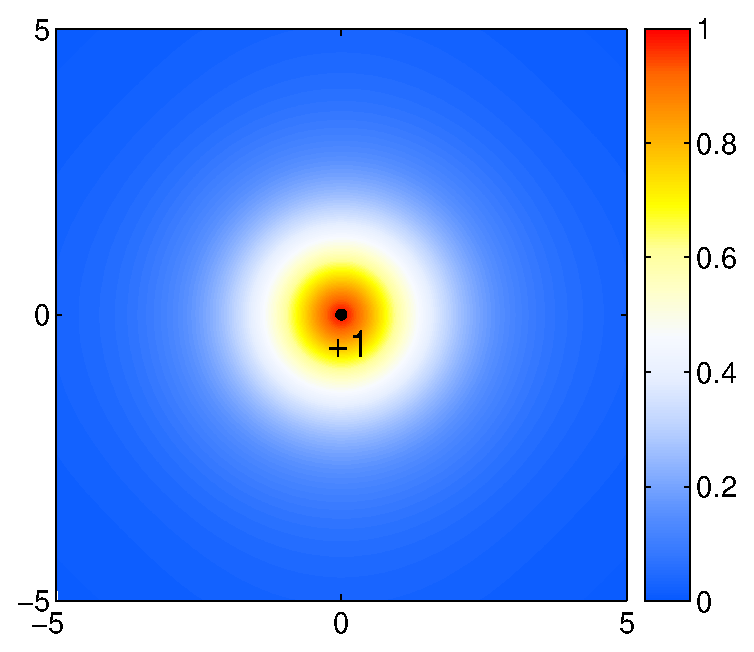
\includegraphics[width=.75\textwidth,bb=148 269 507 577]{results_test1}
%%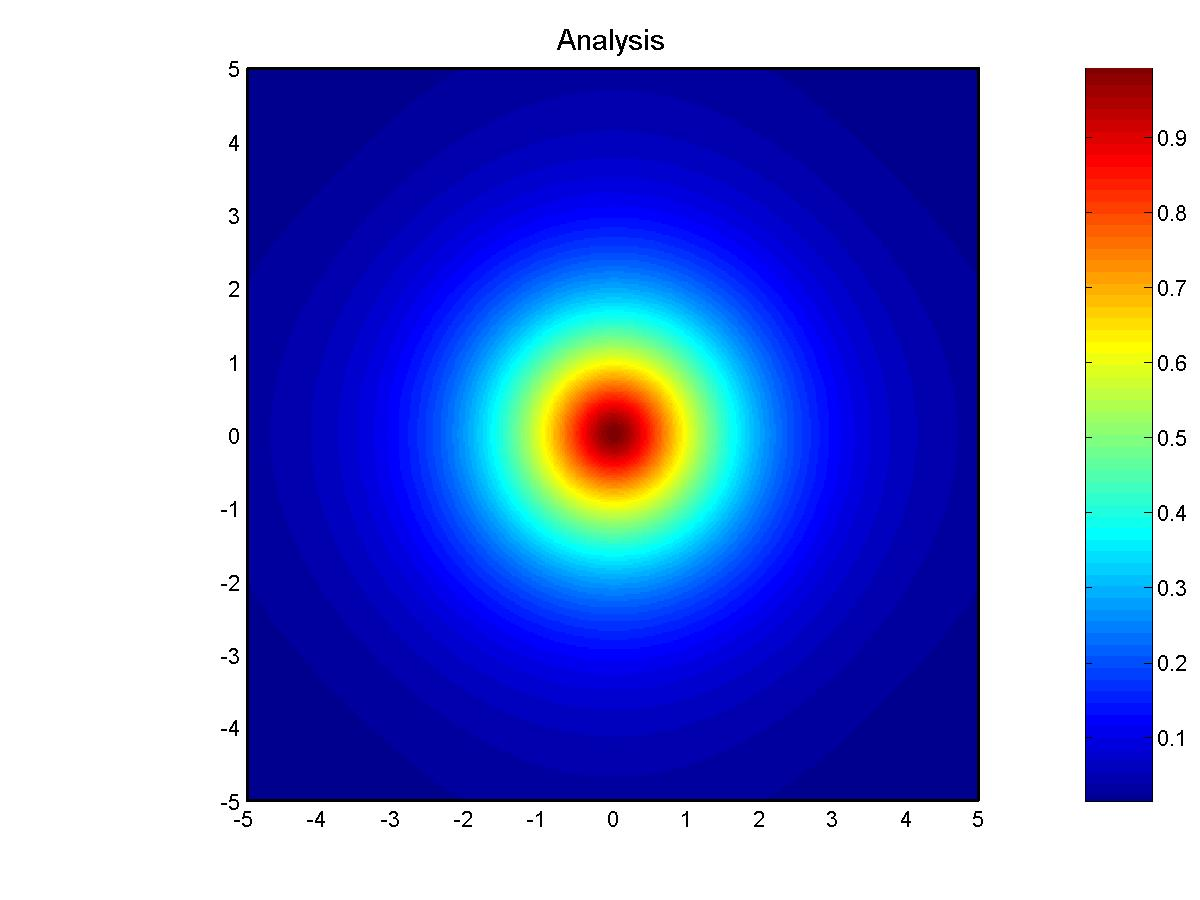
\includegraphics[width=.75\textwidth]{singlepointanalysis}
\caption{Analysis of a single data point with high signal-to-noise ration and no background field.\label{singleanalysis}}
\end{figure}

\begin{figure}[H]
\centering
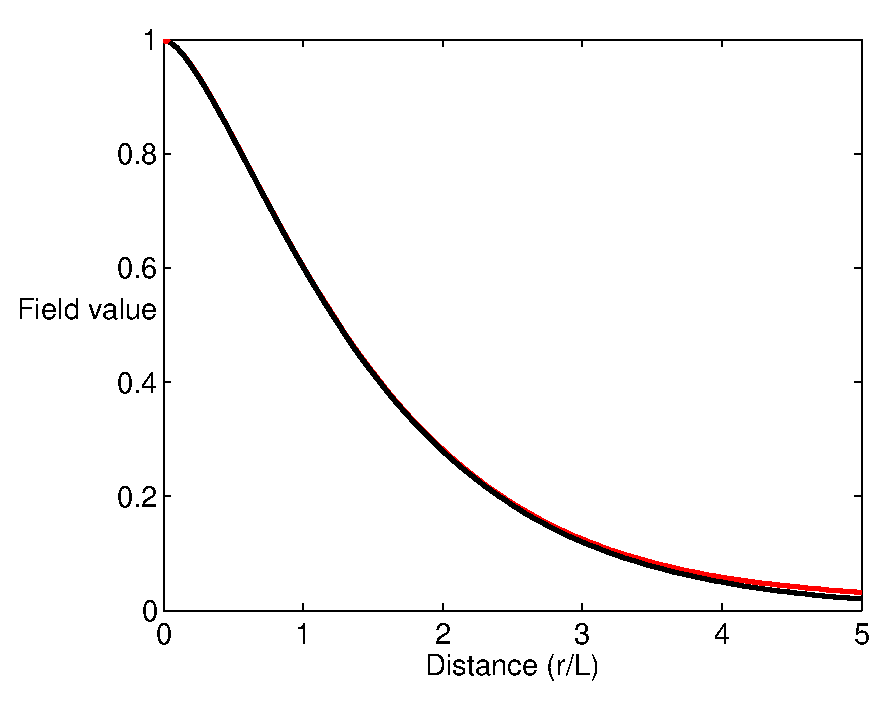
\includegraphics[width=.75\textwidth]{kernelf}
\caption{Kernel function is given in red, while the blue curve comes from the analysis of a single point.\label{kernel1}}
\end{figure}


The Kernel function can be used to calibrate \diva parameters ($\alpha_0, \alpha_1, \mu$) so as to fit observed covariance functions. This principle is used by the tool \command{divafit} which helps one to estimate the correlation length (see Section~\ref{sec:divafit}).

It can also be used for specifying the covariance for error calculations (Chapter~\ref{chap:error}).


\subsection{Comparison OI--VIM}
%-----------------------------------------

\citet{RIXEN00} compared the two methods by testing quasi-synoptic salinity data. Results showed that the main differences between OA and VIM occur in coastal areas and around islands ($\mathcal{O}(0.10)$), whereas the differences range from $-0.01$ to $0.02$ within the domain. The same conclusions were drawn when they compared OI and VIM in the case of climatological data set: both fields were nearly identical, except in the vicinity of the coasts (differences of up to 0.1).

A summary of the main characteristics of the two methods is found in Tab.~\ref{tabOAVIM}.


\begin{table}[htpb]
\caption{Statistical equivalence between OI and VIM (from \citet{RIXEN00})\label{tabOAVIM}}
\begin{tabular*}{0.99\textwidth}{@{\extracolsep{\fill}}lll}
\toprule
											&		OI	& VIM \\
\midrule
Minimization \rule{0pt}{3ex}	& $e^{2}(\mathbf{r})= \overline{ [\varphi(\mathbf{r})-\varphi_{t}(\mathbf{r})]^{2}}$ 	& $J[\varphi]=\sum_{i=1}^{N_d}\mu_{i}[d_{i}-\phi(\mathbf{r_{i}})]^{2}+\left\|\varphi\right\|^{2}$							\\
Solution						& $\varphi(\mathbf{r})= \transp{\mathbf{c}}(\mathbf{r})\mathbf{D}^{-1}\mathbf{d}$			& 
$\varphi(\mathbf{r})= \transp{\mathbf{c}}(\mathbf{r})\mathbf{D}^{-1}\mathbf{d}$												\\
Data correlation				& $[\mathbf{D}]_{ij}=\signal^{2} c(\mathbf{r_{i}},\mathbf{r_{j}})+\noise^{2}\delta_{ij}$& $[\mathbf{D}]_{ij}=K(\mathbf{r_i},\mathbf{r_j})+(1/\snr)\delta_{ij}$														\\
Data-field covariance 			& $[\mathbf{c}]_{i}=\signal^{2} c(\mathbf{r},\mathbf{r_{i}})$							& $[\mathbf{c}]_{i}=K(\mathbf{r},\mathbf{r_{i}})$																			\\
\bottomrule
\end{tabular*}
\end{table}

%-------------------------------------------------------------
\subsection{Comparison between the spatial interpolation methods}
%-------------------------------------------------------------

Table~\ref{tabdata} compares characteristics of different spatial interpolation methods: 
\begin{itemize}
\item the error minimization ($\min( \varepsilon^2)$),
\item the extension to 3 dimensions (3-D), 
\item the multivariate analysis, 
\item the number of operations per analysis, 
\item the error estimate ($\varepsilon(\mathbf{r})$),
\item \textit{a priori} known parameters, 
\item the control parameters and 
\item the treatment of anisotropy. 
\end{itemize} 

All the methods compared here are base on a minimisation of the error estimate except the Cressman method \citep{CRESSMAN59}. OI and VIM are similar methods: they use the same control parameters and require similar a priori information. To work in 3-D and in multivariate mode, VIM needs a few adaptations. 
The main difference concerns the number of operations, which is almost independent on the number of data for VIM.

\begin{table}[htpb]
\caption{Characteristics of different methods of data analysis. $\bullet$ denote available features in the interpolation method, ($\bullet$) indicate that the feature is available with some adaptations. $\varepsilon(\mathbf{r})$ is the error estimate, $N_d$ the number of data points, $N_a$ the number of grid points for analysis, $N$ the number of EOFs, $L$ the correlation length and $\signal^2/ \noise^2$ the signal-to-noise ratio.\label{tabdata}}
\begin{tabular*}{0.99\textwidth}{@{\extracolsep{\fill}}lcccccccc}
\toprule
Method   & $\min(\noise^2)$	& 3-D       & Multivar & Ops/anal.        & $\noise(\mathbf{r})$& \textit{a priori}& C.V. & anis. \\ 
\midrule
Cressman &              	& $\bullet$& $\bullet$& $N_d N_a$        &                & $w(r/L)$   &($L$) & ($\bullet$) 			\\ 
OI    	 &   $\bullet$    	& $\bullet$& $\bullet$& $N_d^3+ N_d N_a$ & $\bullet$      & $c(r/L)$   & $L,\sigma^2/\noise^2$&($\bullet$)	\\ 
{\bf VIM}&   $\bullet$      &($\bullet$)& ($\bullet$)& $N_a^{5/2}$   & $\bullet$      & $K(r/L)$   & $L,\sigma^2/\noise^2$&($\bullet$)	\\
DINEOF   &  ($\bullet$)     & $\bullet$ &  $\bullet$ & $N_a^{5/4}$   & $\bullet$  	  &  --		   & $N$               & $\bullet$	\\ 
\bottomrule
\end{tabular*}
\end{table}

\section{Additional tools}
% ------------------------

\diva software is provided with additional tools designed for parameters adjustment, quality control of results and other physical constraints in the analysis.

\subsection{Automatic estimation of analysis parameters}
%-------------------------------------------------------

The correlation length can be estimated, based on the dataset itself. The method performs a least-square fit of the data covariance function with a theoretical function. 

The signal-to-noise ratio $\snr=\frac{\signal^{2}}{\noise^{2}}$ is estimated with a Generalized Cross-Validation (GCV). GCV allows estimating global errors and calibration of the analysis parameters. 

The tools will be further explained in Chapter~\ref{chap:analysisparameters}.
 
\subsection{Additional physical constraint}
%------------------------------------------

In the base formulation of \diva, the cost function contains a term relative to the regularity of the reconstructed field and a term relative to the proximity to the observations. We will see in Chapter~\ref{chap:advection} that physics (advection, diffusion, source terms) can be added in the cost function.

%--------------------------------------
\subsection{Multi-dimensional analysis}
%--------------------------------------

In order to perform three-dimension analysis (horizontal coordinates and depth), the solution is to applying successive analysis in horizontal layers, from the deeper to the shallower layer. A set of scripts (\command{diva3D*}) are designed to perform such analysis in an automatic way.

However, the reconstruction of three-dimensional fields of temperature and salinity by stacking of layers of analysed fields may lead to unstable density fields. An algorithm has been implemented in \diva in order to remove these instabilities.

These topics are described in Chapter~\ref{chap:godiva}.


\subsection{DINEOF\label{sec:DINEOF}}
%-----------------------------------

\diva is mainly designed to work with in situ data, characterized by a scattered spatial distribution. When dealing with satellite images, the spatial interpolation can be made in a clever way, by using the information contained in the satellite images acquired before in the same region. This idea is implemented in Data INterpolating Empirical Orthogonal Function \citep[DINEOF;][]{BECKERS03,ALVERA05}\index{DINEOF}.

This tool is designed to exploit repeated observations with missing data (e.g., a series of collocated satellite images with clouds). 
For more details about DINEOF, please consult \url{http://modb.oce.ulg.ac.be/mediawiki/index.php/DINEOF} and the other references describing the method: \citet{ALVERA05,ALVERA07,ALVERA09,BECKERS06}.


